\documentclass[a4paper, 12pt]{article}
\usepackage[total={17cm,25cm}, top=2.5cm, left=2.5cm, right=2.5cm,  includefoot]{geometry}
\usepackage[utf8]{inputenc}
\usepackage{array}
\usepackage{multirow}
\usepackage{hhline}
\usepackage{gensymb}
\usepackage{graphicx}
\graphicspath{ {} }
\usepackage[czech]{babel}
\usepackage{enumitem}
\usepackage{pdfpages}
\usepackage{amsmath}
\usepackage{verbatim}
\usepackage{listings}
\usepackage{hyperref}
\usepackage{amssymb}
\usepackage{hyperref}

\def\UrlBreaks{\do\/\do-\do.\do=\do_\do?\do\&\do\%\do\a\do\b\do\c\do\d\do\e\do\f\do\g\do\h\do\i\do\j\do\k\do\l\do\m\do\n\do\o\do\p\do\q\do\r\do\s\do\t\do\u\do\v\do\w\do\x\do\y\do\z\do\A\do\B\do\C\do\D\do\E\do\F\do\G\do\H\do\I\do\J\do\K\do\L\do\M\do\N\do\O\do\P\do\Q\do\R\do\S\do\T\do\U\do\V\do\W\do\X\do\Y\do\Z\do\0\do\1\do\2\do\3\do\4\do\5\do\6\do\7\do\8\do\9}


\usepackage{listings}
\usepackage{color}
 
\definecolor{codegreen}{rgb}{0,0.6,0}
\definecolor{codegray}{rgb}{0.5,0.5,0.5}
\definecolor{codepurple}{rgb}{0.58,0,0.82}
\definecolor{backcolour}{rgb}{0.95,0.95,0.92}
 
\lstdefinestyle{mystyle}{
    backgroundcolor=\color{backcolour},   
    commentstyle=\color{codegreen},
    keywordstyle=\color{magenta},
    numberstyle=\tiny\color{codegray},
    stringstyle=\color{codepurple},
    basicstyle=\footnotesize,
    breakatwhitespace=false,         
    breaklines=true,                 
    captionpos=b,                    
    keepspaces=true,                 
    numbers=left,                    
    numbersep=5pt,                  
    showspaces=false,                
    showstringspaces=false,
    showtabs=false,                  
    tabsize=2
}
 
\lstset{style=mystyle}


\pagestyle{empty} % vypne číslování stránek




%\usepackage[OT2,OT1]{fontenc}
\newcommand\cyr
{
\renewcommand\rmdefault{wncyr}
\renewcommand\sfdefault{wncyss}
\renewcommand\encodingdefault{OT2}
\normalfont
\selectfont
}
\DeclareTextFontCommand{\textcyr}{\cyr}
\def\cprime{\char"7E }
\def\cdprime{\char"7F }
\def\eoborotnoye{\char’013}
\def\Eoborotnoye{\char’003}

\setlength\parindent{0pt}

\begin{document}



\begin{titlepage}
\begin{center}
\noindent
\Large \textbf{České vysoké učení technické v Praze }\\ Fakulta stavební
\vspace{5cm}

\Large

%vložení loga cvut
%\begin{figure}[h!]
%	\centering
%	\includegraphics[width=7cm]{logo.png}
%\end{figure}

\vspace{4cm}

155UZPD: Semestrální projekt \\
\Huge

\textbf{MMDOS - Síťové analýzy PID}
\vspace{11cm}

\large
Únor 2019 \hspace{5cm} Petra M. Millarová, Michael Kala\\

\end{center}

\end{titlepage}




\pagestyle{plain}     % zapne obyčejné číslování
\setcounter{page}{1}  % nastaví čítač stránek znovu od jedné

%\tableofcontents
%\newpage

\section{Cíl projektu}
Cílem semestrálního projektu bylo vytvoření konzolové aplikace MMDOS, jež provádí síťové analýzy nad daty PID za využití pgRouting, extenze PostGISu. Uživatel má možnost zadat výchozí a cílovou adresu, aplikace vyhledá nejbližší zastávky hromadné dopravy, provede síťovou analýzu a vrátí nejkratší cestu. Uživateli se poté zobrazí seznam zastávek a linek, které by měl po cestě využít.

\newpage
\section{Data}
\begin{itemize}
	\item Adresní místa RÚIAN Hlavního města Prahy, staženo z Nahlížení do KN (dokumentace: \url{http://vdp.cuzk.cz/vymenny_format/csv/ad-csv-struktura.pdf})
	\item Síť tras linek Pražské integrované dopravy, staženo z portálu Opendata Hlavního města Prahy (dokumentace: \url{http://www.geoportalpraha.cz/cs/fulltext_geoportal?id=6F576389-385E-4E38-831A-8DE6EFB52C3A#.XErv8stKiV4})
	\item Zastávky PID - jednotlivé označníky, staženo z portálu Opendata Hlavního města Prahy (dokumentace: \url{http://www.geoportalpraha.cz/cs/fulltext_geoportal?id=63EF19FE-C2FB-4FC2-8C2D-EEBB72C6B81A#.XErxJ8tKiV4})
\end{itemize}

\newpage
\section{Zpracování dat}
\subsection{Adresní místa RUIAN}
Data byla stažena ve formátu \texttt{csv}. Následně pomocí jazyka AWK byl v shellu soubor upraven, aby obsahoval pouze potřebná data (resp. byl vytvořen nový soubor):
\begin{lstlisting}[language=awk]
awk -F \; '{print $11";"$13";"$14";"$15";"$17";"$18}' 20181231_OB_554782_ADR.csv > ruian_adr.csv
\end{lstlisting}

Ponechány byly sloupce ulice, číslo domovní, číslo orientační, číslo orientační znak (a, b..) a souřadnice x, y v S-JTSK. 

Dále byla v databázi na geo102 vytvořena a naplněna tabulka \texttt{adr} (včetně geometrie) pomocí dávkového souboru \texttt{adr.sql} puštěného pomocí příkazu:

\begin{lstlisting}[language=bash]
psql -h geo102.fsv.cvut.cz -d pgis_uzpd -U uzpd18_a -f adr.sql	
\end{lstlisting}

Obsah dávkového souboru:

\begin{lstlisting}[language=sql]
CREATE TABLE adr(
	gid serial NOT NULL,
	ulice VARCHAR(50),
	c_domovni INTEGER,
	c_orientacni INTEGER,
	co_znak VARCHAR(2),
	y REAL,
	x REAL,
	geom geometry);
	
\copy adr(ulice, c_domovni, c_orientacni, co_znak, y, x) FROM '../ruian_adr.csv' DELIMITER ';' CSV HEADER encoding 'windows-1250';

UPDATE adr SET geom = ST_GeomFromText('POINT(-'||y||' -'||x||')',5514);

DELETE FROM adr WHERE geom IS NULL;

\end{lstlisting}

Aby byly názvy ulic importovány správně s diakritikou, bylo třeba nastavit kódování na uvedenou hodnotu \texttt{windows-1250}. Zároveň byla pro potřeby projektu z dat vymazána adresní místa bez geometrie.

\subsection{Data PID}
Data zastávek a tras linek PID byla stažena ve formátu \texttt{shp}. Pro import dat do databáze byl využit nástroj PostGISu \texttt{shp2pgsql}, jež konvertuje soubory ve formátu \texttt{shp} do databázových tabulek. Toto bylo vykonáno pomocí příkazu (v shellu):

\begin{lstlisting}[language=bash]
shp2pgsql -s 5514 -D -I DOP_PID_TRASY_TS_L.shp | psql -h geo102.fsv.cvut.cz -d pgis_uzpd -U uzpd18_a
\end{lstlisting} 
 
A přímo v databázi byl změněn název vytvořené tabulky:

\begin{lstlisting}[language=sql]
ALTER TABLE dop_pid_trasy_ts_l RENAME TO trasy;
\end{lstlisting} 

Pro potřeby našeho projektu nebyly nutné údaje o nočních linkách, proto byly tyto řádky smazány (soubor \texttt{mazani\_nocnich.sql}): 
\begin{lstlisting}[language=sql]
DELETE FROM trasy 
WHERE (l_metro_n IS NULL
	OR l_tram_n IS NOT NULL
	OR l_bus_n IS NOT NULL
	OR l_lan_n IS NOT NULL
	OR l_vlak_n IS NOT NULL
	OR l_lod_n IS NOT NULL
	AND l_metro IS NULL
	AND l_tram IS NULL
	AND l_bus IS NULL
	AND l_lan IS NULL 
	AND l_vlak IS NULL 
	AND l_lod IS NULL);
\end{lstlisting} 

Analogicky se postupovalo u zastávek:

\begin{lstlisting}[language=bash]
shp2pgsql -s 5514 -D -I DOP_PID_ZASTAVKY_TS_B.shp| psql -h geo102.fsv.cvut.cz -d pgis_uzpd -U uzpd18_a
\end{lstlisting} 

\begin{lstlisting}[language=sql]
ALTER TABLE dop_pid_zastavky_ts_b RENAME TO zastavky;
\end{lstlisting} 

U zastávek byly taktéž smazány řádky obsahující pouze údaje o nočních linkách:
\begin{lstlisting}[language=sql]
DELETE FROM zastavky WHERE zast_denno = 2;
\end{lstlisting} 

Vzhledem k prapodivnosti sloupce \texttt{zast\_id}, kde se ukázalo, že více zastávek s různými názvy a různým umístěním mají stejné ID, se autoři rozhodli použít sloupec \texttt{zast\_uzel} jako identifikátor zastávky, protože byla hodnota stejná pro všechny položky se stejným názvem zastávky. Sloupec bylo třeba přetypovat na typ \texttt{INTEGER} následujícím příkazem: 

\begin{lstlisting}[language=sql]
ALTER TABLE zastavky 
ALTER COLUMN zast_uzel_ TYPE INTEGER 
USING CAST(zast_uzel_ AS INTEGER);
\end{lstlisting} 

\section{Topologie}
\subsection{Hrany}
Vzhledem ke komplikacím zmiňovaným v předchozí kapitole se autoři rozhodli vytvořit topologii bez použití funkce z extenze pgRouting k tomu určené -  \texttt{pgr\_createTopology}. Nejprve byly do tabulky \texttt{trasy} přidány sloupce \texttt{source} a \texttt{target} a vytvořen prostorový index (soubor \texttt{topo.sql}): 
\begin{lstlisting}[language=sql]
ALTER TABLE trasy ADD COLUMN "source" integer;
ALTER TABLE trasy ADD COLUMN "target" integer;
CREATE INDEX ON trasy USING gist(geom);
\end{lstlisting} 

Následně byl vytvořen skript v Pythonu, který pomocí prostorového dotazu k začátku i konci každé linie v tabulce \texttt{trasy} vybral nejbližsí bod z tabulky \texttt{zastavky} a vrátil ID jeho uzlu, které pak bylo dosazeno do sloupce \texttt{source}, případně \texttt{target}. Vzhledem k tomu, že geometrickým typem linií v tabulce \texttt{trasy} byl \texttt{MultiLineString} a funkce \texttt{ST\_StartPoint()} resp. \texttt{ST\_EndPoint()} jako argument bere pouze typ \texttt{LineString}, bylo třeba mezi těmito typy provést konverzi.
\newpage
Celý skript (soubor \textit{MMTopology.py}):
\begin{lstlisting}[language=python]
import psycopg2


# connect to database
conn = psycopg2.connect(host="geo102.fsv.cvut.cz",
						database="pgis_uzpd",
						user="uzpd18_a",
						password="a_uzpd18")

cur = conn.cursor()
cur_s = conn.cursor()
cur_e = conn.cursor()

# Select starting points
cur_s.execute("SELECT DISTINCT ON(t.gid) t.gid, z.zast_uzel_ FROM trasy t, zastavky z WHERE ST_DWithin(ST_StartPoint(ST_LineMerge(t.geom)), z.geom, 500) AND t.zast_id_od = z.zast_id")

# Select end points
cur_e.execute("SELECT DISTINCT ON(t.gid) t.gid, z.zast_uzel_ FROM trasy t, zastavky z WHERE ST_DWithin(ST_EndPoint(ST_LineMerge(t.geom)), z.geom, 500) AND t.zast_id_ka = z.zast_id")

sp = cur_s.fetchone()
ep = cur_e.fetchone()
i = 0

# loop through starting and ending points, update source and target
while sp is not None or ep is not None:
	if sp is not None:
		cur.execute("UPDATE trasy SET source = {} WHERE gid = {}".format(sp[1],sp[0]))
	if ep is not None:
		cur.execute("UPDATE trasy SET target = {} WHERE gid = {}".format(ep[1],ep[0]))
	sp = cur_s.fetchone()
	ep = cur_e.fetchone()		

conn.commit()

cur_s.close()
cur_e.close()
cur.close()

if conn is not None:
	conn.close()
\end{lstlisting}

Počet řádků v tabulce trasy se pohybuje kolem 85 000, skript běžel několik desítek minut. 

\newpage

\subsection{Uzly}
Následně byla vytvořena tabulka uzlů pomocí funkce \textit{pgr\_createVerticesTable}. Sloupec \texttt{the\_geom} byl přejmenován na \texttt{geom} (soubor \texttt{uzly.sql}):
\begin{lstlisting}[language=sql]
SELECT pgr_createVerticesTable('trasy','geom','source','target');
ALTER TABLE trasy_vertices_pgr rename column the_geom to geom;
\end{lstlisting} 

\section{Konzolová aplikace}
\subsection{Popis výpočtu}
V jazyce Python byl vytvořen skript (soubor \texttt{MMDOS.py}), který na vstup uživatele provádí síťovou analýzu za využití Dijkstrova algoritmu implementovaného v pgRouting jako funkce \texttt{pgr\_dijkstra}. Postup výpočtu je následující:
\begin{enumerate}
\item Zjištění ID nejbližších zastávek od zadaných adres, aplikace umožňuje uživateli zadat následující kombinace údajů o adresách:
	\begin{itemize}
		\item ulice, č.p./č.o.
		\item ulice, č.p.
		\item ulice, č.o.
		\item ulice
	\end{itemize}
	kdy na základě zadaných údajů je vyhledána adresa jim vyhovující, případně první z adres jim vyhovující.
\item Výpočet nejkratší cesty pomocí Dijstrova algoritmu.
\item Výpis zastávek a linek respektující nejmenší počet přestupů.
	\begin{itemize}
		\item V tabulce \texttt{trasy} jsou pro každý úsek vyjmenovány všechny linky, které na daném úseku poskytují přepravu. Program prochází vytvořenou trasu a vybírá linky s nejmenším počtem přestupů následovně:
			\begin{enumerate}
				\item Průchod všech linek projíždějících první zastávkou (resp. úsekem mezi první a druhou zastávkou), výpočet dosahu každé linky (tedy až o kolik zastávek se lze posunout danou linkou).
				\item Přiřazení čísla linky s nejdelším dosahem (příp. první z linek, které mají shodný nejdelší dosah) k daným zastávkám.
						\begin{itemize}
							\item Vzhledem k přiřazování čísel linek k počátečním bodům  úseků, se číslo linky nepřiřadí k poslední zastávce, do které vybraná linka dosahuje. Toto je využito v dalším kroku.
						\end{itemize}
				\item Opakování kroku (a) a (b) od první zastávky s nepřiřazeným číslem linky.
			\end{enumerate}
	\end{itemize}
\end{enumerate} 

\subsection{Vytvořené SQL funkce}
Pro potřeby konzolové aplikace byly vytvořeny následující SQL funkce (soubor \texttt{funkce.sql}):

\begin{itemize}
\item Funkce pro zjištění názvu zastávky podle zadaného ID.
\begin{lstlisting}[language=sql]
CREATE OR REPLACE FUNCTION FindStationName(id INTEGER)
RETURNS VARCHAR AS $name$
declare 
	name varchar;
BEGIN 
	SELECT z.zast_nazev INTO name FROM zastavky z
	WHERE z.zast_uzel_ = id LIMIT 1; 
	RETURN name;
END;
$name$ LANGUAGE plpgsql;
\end{lstlisting} 

\item Set funkcí pro zjištění ID zastávky, která je nejblíže zadané adrese. První tři funkce jsou uzpůsobeny na zadání názvu ulice a kombinace čísla orientačního, popisného a nebo obou. Poslední z funkcí umožňuje uživateli zadat jen název ulice, přičemž funkce vrací i adresu, ke které bylo hledání nejbližší zastávky vztaženo. U prvních dvou funkcí není třeba vracet celou adresu, jelikož čísla popisná a orientační jsou dle zákona unikátní v rámci ulice (popisné v rámci části obce).

\begin{lstlisting}[language=sql]
CREATE OR REPLACE FUNCTION FindVertexID(cd INTEGER, co INTEGER, u VARCHAR)
RETURNS INTEGER AS $id$
declare 
	id integer;
BEGIN 
	SELECT v.id INTO id FROM adr a, trasy_vertices_pgr v 
	WHERE a.c_domovni = cd 
	AND a.c_orientacni = co 
	AND a.ulice = u
	ORDER BY (a.geom)<->(v.geom) asc limit 1;
	RETURN id;
END;
$id$ LANGUAGE plpgsql;

CREATE OR REPLACE FUNCTION FindVertexIDcd(cd INTEGER, u VARCHAR)
RETURNS INTEGER AS $id$
declare 
	id integer;
BEGIN 
	SELECT v.id INTO id FROM adr a, trasy_vertices_pgr v 
	WHERE a.c_domovni = cd 
	AND a.ulice = u
	ORDER BY (a.geom)<->(v.geom) asc limit 1;
	RETURN id;
END;
$id$ LANGUAGE plpgsql;

CREATE OR REPLACE FUNCTION FindVertexIDori(co INTEGER, u VARCHAR)
RETURNS INTEGER AS $id$
declare 
	id integer;
BEGIN 
	SELECT v.id INTO id FROM adr a, trasy_vertices_pgr v 
	WHERE a.c_orientacni = co
	AND a.ulice = u
	ORDER BY (a.geom)<->(v.geom) asc limit 1;
	RETURN id;
END;
$id$ LANGUAGE plpgsql;

CREATE OR REPLACE FUNCTION FindVertexIDst(u VARCHAR)
RETURNS TABLE(
id BIGINT,
ul VARCHAR,
cp INTEGER,
co INTEGER
	) as $$
BEGIN 
	RETURN QUERY SELECT v.id, a.ulice, a.c_domovni, a.c_orientacni FROM adr a, trasy_vertices_pgr v 
	WHERE a.ulice = u
	ORDER BY (a.geom)<->(v.geom) asc limit 1;
 END; 
$$
LANGUAGE plpgsql;
\end{lstlisting} 
\end{itemize} 

\subsection{Dijskrův algoritmus}
Pro výpis nejkratší cesty byl použit následující příkaz:
\begin{lstlisting}[language=SQL]
SELECT z.zast_nazev, trasy.l_metro, trasy.l_tram, trasy.l_bus, trasy.l_lan, trasy.l_vlak, trasy.l_lod, node
FROM pgr_dijkstra('SELECT gid AS id, source, target, CAST(shape_leng AS REAL) AS cost FROM trasy', id_from, id_to)
JOIN (
	SELECT DISTINCT(zastavky.zast_uzel_), zastavky.zast_nazev FROM zastavky
	) AS z ON node = z.zast_uzel_
LEFT JOIN trasy ON edge = trasy.gid 
ORDER BY seq;
\end{lstlisting}
kde \texttt{id\_from, id\_to} jsou ID počáteční a koncové zastávky. \\
K tabulce výsledků z výpočtu funkcí \texttt{pgr\_dijkstra} byla přes sloupec \texttt{zast\_uzel\_} připojena tabulka \texttt{zastavky}, ze které byl vypsán název zastávky. Připojena byla též tabulka \texttt{trasy} pro zobrazení linek, které daným místem projíždějí. Protože poslední uzel nemá žádnou navazující hranu, ale musí být také vypsán, byl použit \texttt{LEFT JOIN}, který zachovává všechny údaje z původní tabulky. Nakonec byl výstup seřazen podle atributu \texttt{seq}, jež udává pořadí zastávek v nalezené trase.
\newpage
\subsection{Ukázka aplikace}
Aplikace lze spustit spuštěním skriptu \texttt{MMDOS.py} případně v OS Linux pomocí stand-alone spustitelného souboru \texttt{MMDOS} (v přílohách).
\begin{figure}[h!]
 \centering
 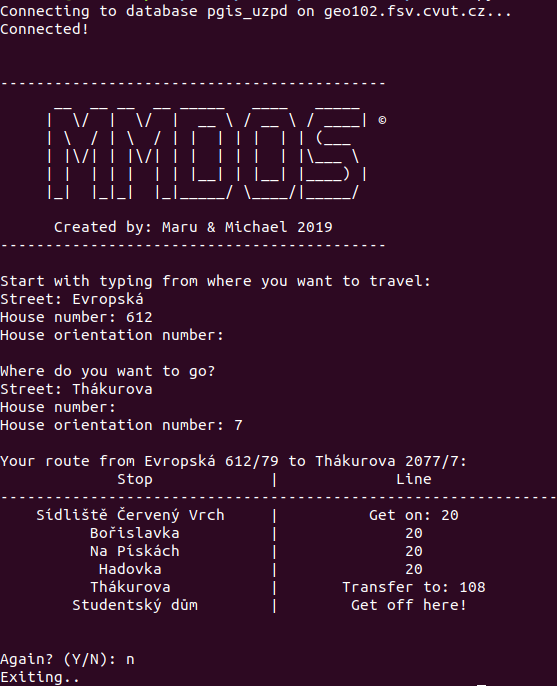
\includegraphics[scale=0.5]{ukazka.png}
\end{figure}


\newpage
\section{Závěr}
\subsection{Zhodnocení}
Byla vytvořena konzolová aplikace pro vyhledávání spojů PID v závislosti na zadané adrese počátečního a cílového místa. Aplikace respektuje nejmenší počet přestupů. \\
Při zpracování dat se vyskytlo několik problémů, zejména u dat poskytovaných na serveru Opendata, kde docházelo k případům, že několik zastávek mělo stejné "unikátní ID", přestože se nejmenovaly stejně a ani se nenacházely na stejném dopravním uzlu. Stejná ID byla použita v datové sadě s linkami PID u ID počátečních a koncových bodů jednotlivých úseků linek. Toto vyústilo v problém, kdy docházelo k chybnému přiřazení zastávek k příslušným úsekům linek. Tento problém byl vyřešen pomocí prostorového dotazování na nejbližší zastávky k daným bodům. \\
Dalším problémem byla přítomnost záznamů linek s nočními spoji. To způsobovalo chybné vyhledávání nejkratších tras. Toto bylo vyřešeno vymazáním těchto údajů z tabulky. \\

\subsection{Náměty na vylepšení}
\begin{itemize}
	\item Ocenění tras např. podle typu dopravy - současný model hledá nejkratší trasu bez ohledu na přestupy
	\item Přidání možnosti nočního cestování
	\item Přidání jízdních řádů
\end{itemize}

\newpage
\section{Přílohy}
\begin{itemize}
	\item Import adres do databáze - \texttt{adr.sql}
	\item Mazání údajů o nočních linkách - \texttt{mazani\_nocnich.sql}
	\item Topologie tras (přidání sloupců) - \texttt{topo.sql}
	\item Skript pro topologii tras - \texttt{MMTopology.py}
	\item Vytvoření tabulky s uzly - \texttt{uzly.sql}
	\item Skript MMDOS - \texttt{MMDOS.py}
	\item Vytvořené SQL funkce - \texttt{funkce.sql}
	\item Stand-alone aplikace - \texttt{MMDOS}
\end{itemize}


\newpage
\section{Zdroje}

\begin{itemize}
\item Nahlížení do KN, aplikace ČÚZK - \url{https://nahlizenidokn.cuzk.cz/} 

\item Portál pro Otevřená data hlavního města Prahy - \url{http://opendata.praha.eu/}

\item Upload csv tabulky do databáze - \url{http://www.postgresqltutorial.com/import-csv-file-into-posgresql-table/}

\item Tvorba topologie pomocí pgRouting - \url{http://docs.pgrouting.org/latest/en/pgr\_createTopology.html}

\item Tvorba nové tabulky uzlů - \url{http://docs.pgrouting.org/latest/en/pgr\_createVerticesTable.html}

\item Funkce pro vyhledání nejkratší trasy - \url{http://docs.pgrouting.org/latest/en/pgr\_dijkstra.html}

\end{itemize}

\end{document}



 